\subsection{Overbelægning}
Definitionen af overbelægning er en overstigelse af indlagte patienter på en given afdeling ift. tilgængelige sengepladser. Overbelægning er estimeret til at være 85\% af det samlede antal sengepladser, herefter er det påvist at sandsynligheden for hospitalets mortalitet \fxnote{hyppigheden af dødsfald i en befolkning angives ved forholdet mellem antallet af døde inden for et givet tidsrum og størrelsen af befolkningen.} stiger 9\% sammenlignet med underbelægning. \citep{dodlighed2014} For at mindske konsekvenser af dette er det vigtigt at finde en ligevægt mellem over- og underbelægning.  

\noindent
Antallet af patienter, der indlægges varierer fra måned til måned, hvorfor tilgængeligheden af sengepladser også variererer. Dette gør sig gældende for flere forskellige afdelinger. Dette fremgår af \autoref{fig:overbelaegning_ran}.

\begin{figure}[H]
\centering
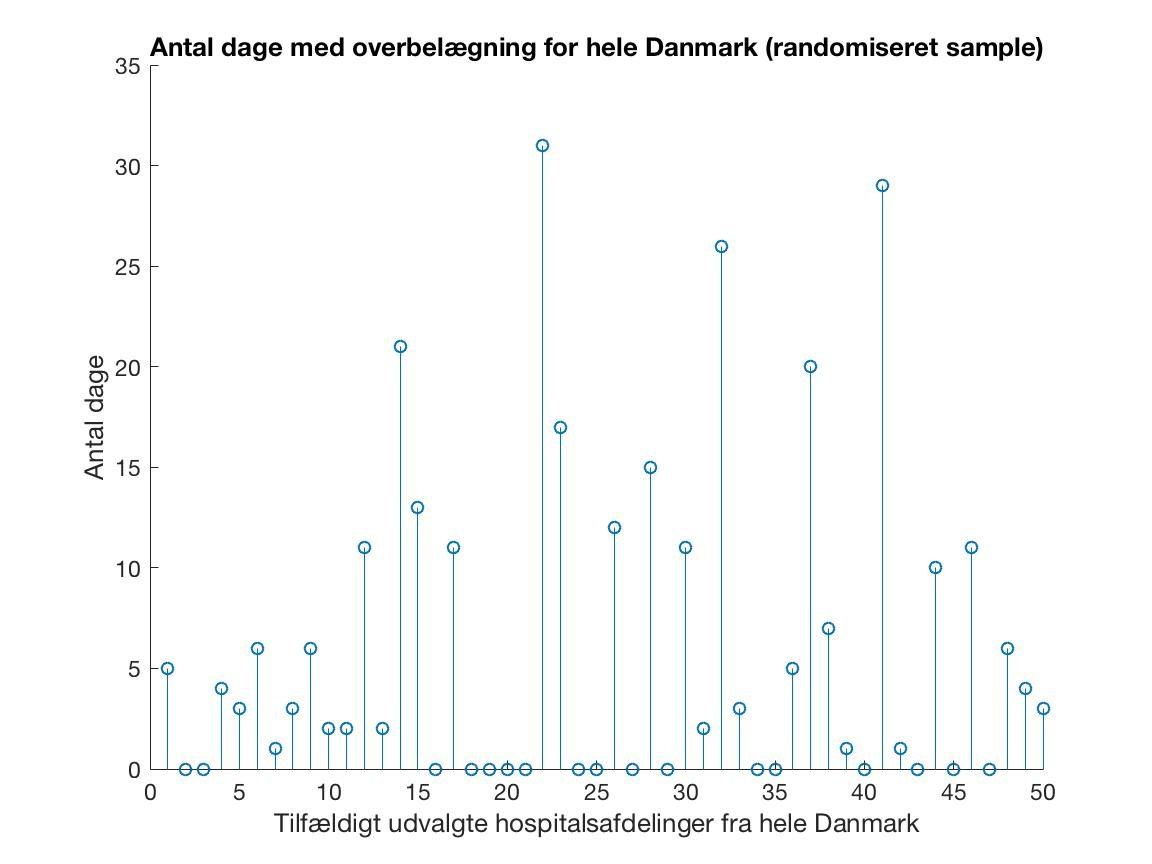
\includegraphics[width=1\textwidth]{figures/overbelaegning_ran.fig}
\caption{Antal dage med overbelægning for hele Danmark udarbejdet med tilfældig udvalgte hospitalsafdelinger fra hele Danmark. De randomiserede data er taget over en periode på 6 måneder.}
\label{fig:overbelaegning_ran}
\end{figure}


\begin{figure}[H]
\centering
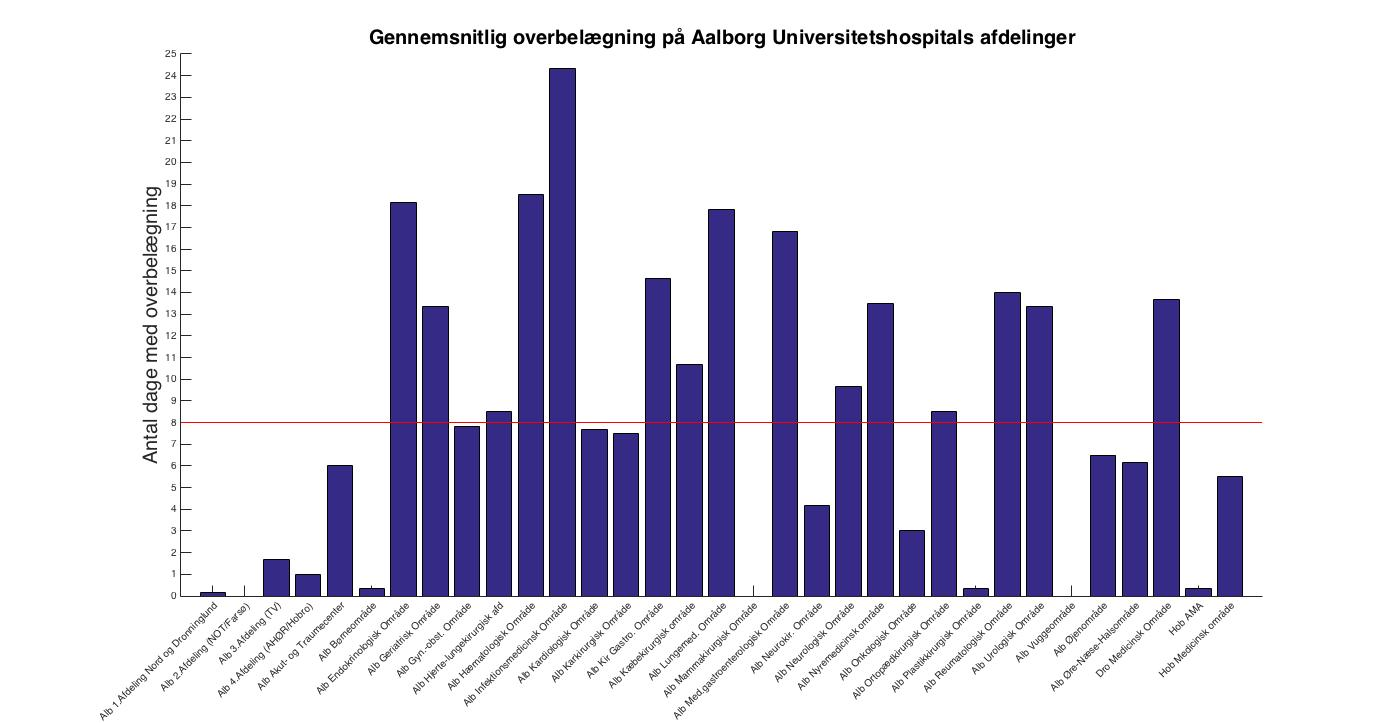
\includegraphics[width=1\textwidth]{figures/overbelaegning_AUH.fig}
\caption{Gennemsnitlig overbelægning på Aalborg Universitetshospitals afdelinger målt i antal dage. Målingerne er taget for samtlige afdelinger på Aalborg Universitetshospital og er taget over en periode på 6 måeneder}
\label{fig:overbelaegning_AUH}
\end{figure}